\documentclass[xcolor=dvipsnames]{beamer}
\usepackage[T1]{fontenc}
\usepackage[utf8]{inputenc}
\usepackage[english,slovak]{babel}

\usepackage{amsmath}
\usepackage{amsthm}
\usetheme{Pittsburgh}
\useoutertheme{shadow}

\usepackage{graphicx}
\usepackage{caption}
\usepackage{subcaption}

\usepackage[]{algorithm2e}
\usepackage{listings}
 \setbeamercovered{transparent}
 \usepackage{cuted}
\usepackage[export]{adjustbox}
\usepackage{mathtools}

\usepackage{lipsum}
\usepackage{verbatim}

\newcommand\Wider[2][3em]{%
\makebox[\linewidth][c]{%
  \begin{minipage}{\dimexpr\textwidth+#1\relax}
  \raggedright#2
  \end{minipage}%
  }%
}




\iftrue

\usetheme{Warsaw}

\setbeamercolor{normal text}{fg=white,bg=black!90}
\setbeamercolor{structure}{fg=white}

\setbeamercolor{alerted text}{fg=red!85!black}

\setbeamercolor{item projected}{use=item,fg=black,bg=item.fg!35}

\setbeamercolor*{palette primary}{use=structure,fg=structure.fg}
\setbeamercolor*{palette secondary}{use=structure,fg=structure.fg!95!black}
\setbeamercolor*{palette tertiary}{use=structure,fg=structure.fg!90!black}
\setbeamercolor*{palette quaternary}{use=structure,fg=structure.fg!95!black,bg=black!80}

\setbeamercolor*{framesubtitle}{fg=white}

\setbeamercolor*{block title}{parent=structure,bg=black!60}
\setbeamercolor*{block body}{fg=black,bg=black!10}
\setbeamercolor*{block title alerted}{parent=alerted text,bg=black!15}
\setbeamercolor*{block title example}{parent=example text,bg=black!15}

\fi



%-------------------------------------------------------------------------------------
\title{\bf Reinforcement learning}
\author{Michal CHOVANEC, PhD}


%\setbeamertemplate{footline}[frame number]{}
\setbeamertemplate{navigation symbols}{}


\date[EURP]{}
\begin{document}

\begin{frame}
\titlepage

\vspace{-50pt}
  \begin{figure}[htc]
    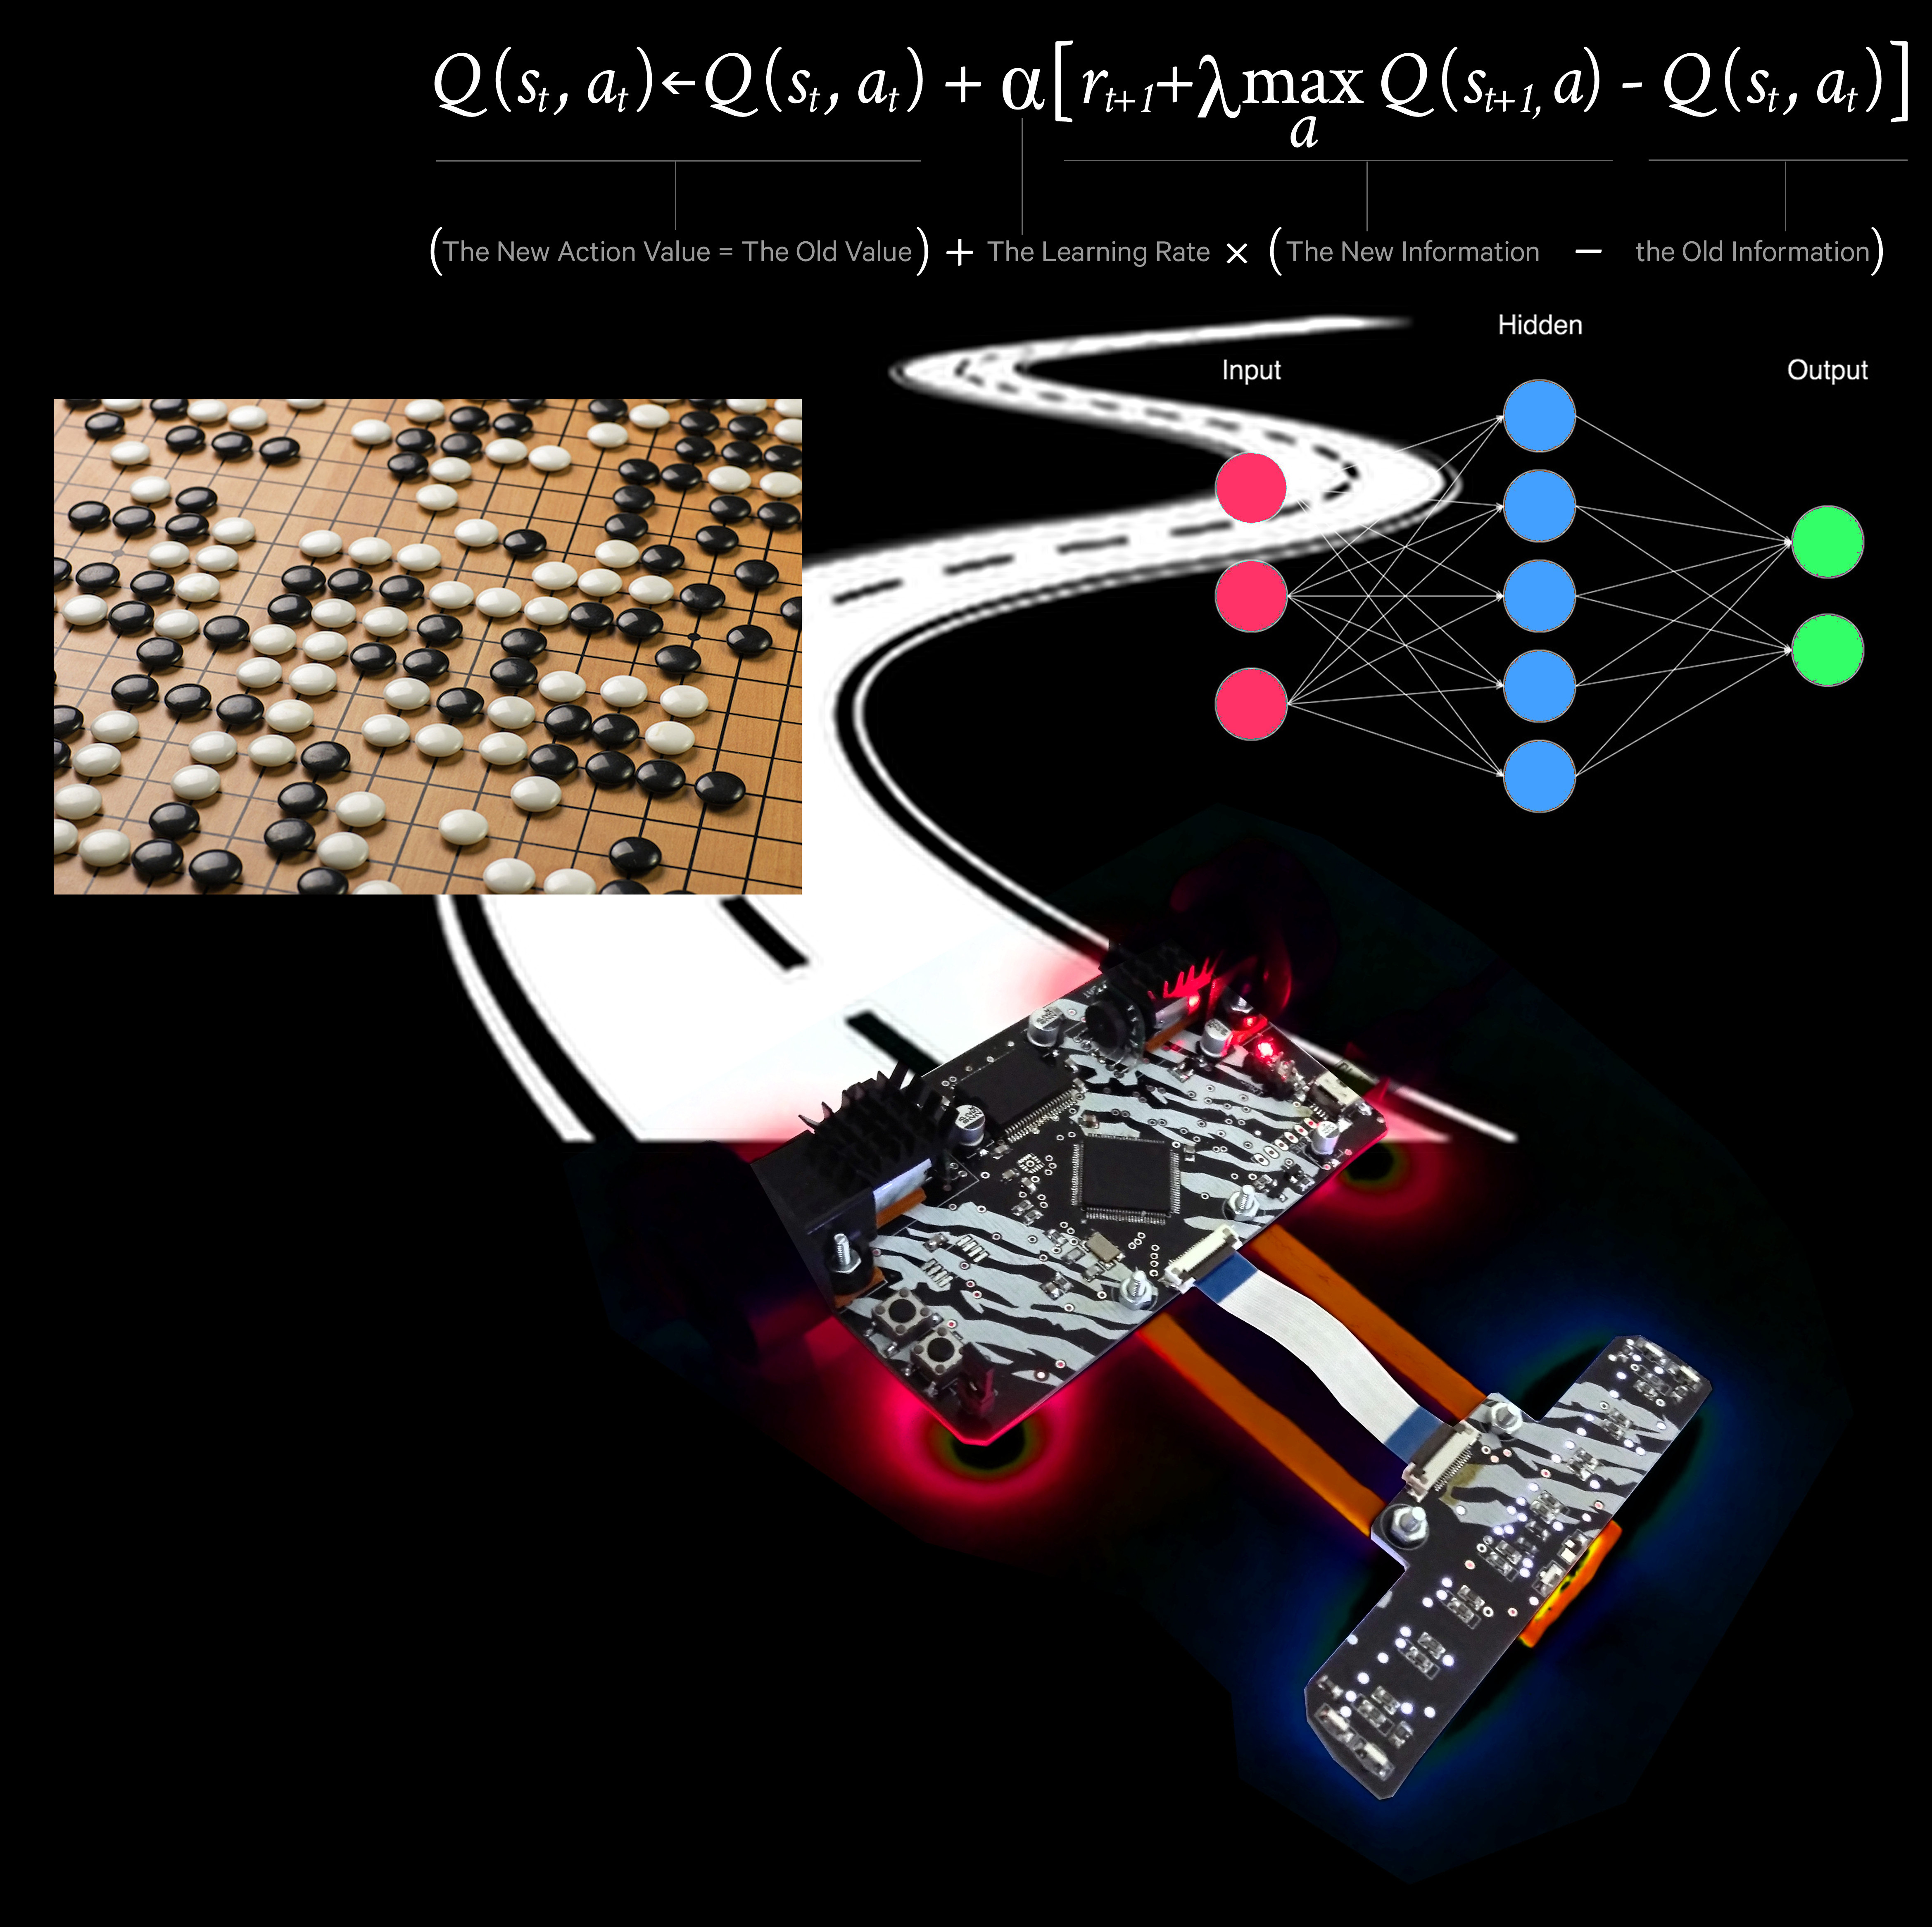
\includegraphics[scale=0.04]{../../pictures/rl_square.jpg}
  \end{figure}


\end{frame}


\begin{frame}{\bf Reinforcement learning}

\begin{itemize}
  \item learn from punishment and rewards
  \item learn to play a game with unknow rules
\end{itemize}

\begin{columns}
\begin{column}{0.5\textwidth}

  \begin{figure}
    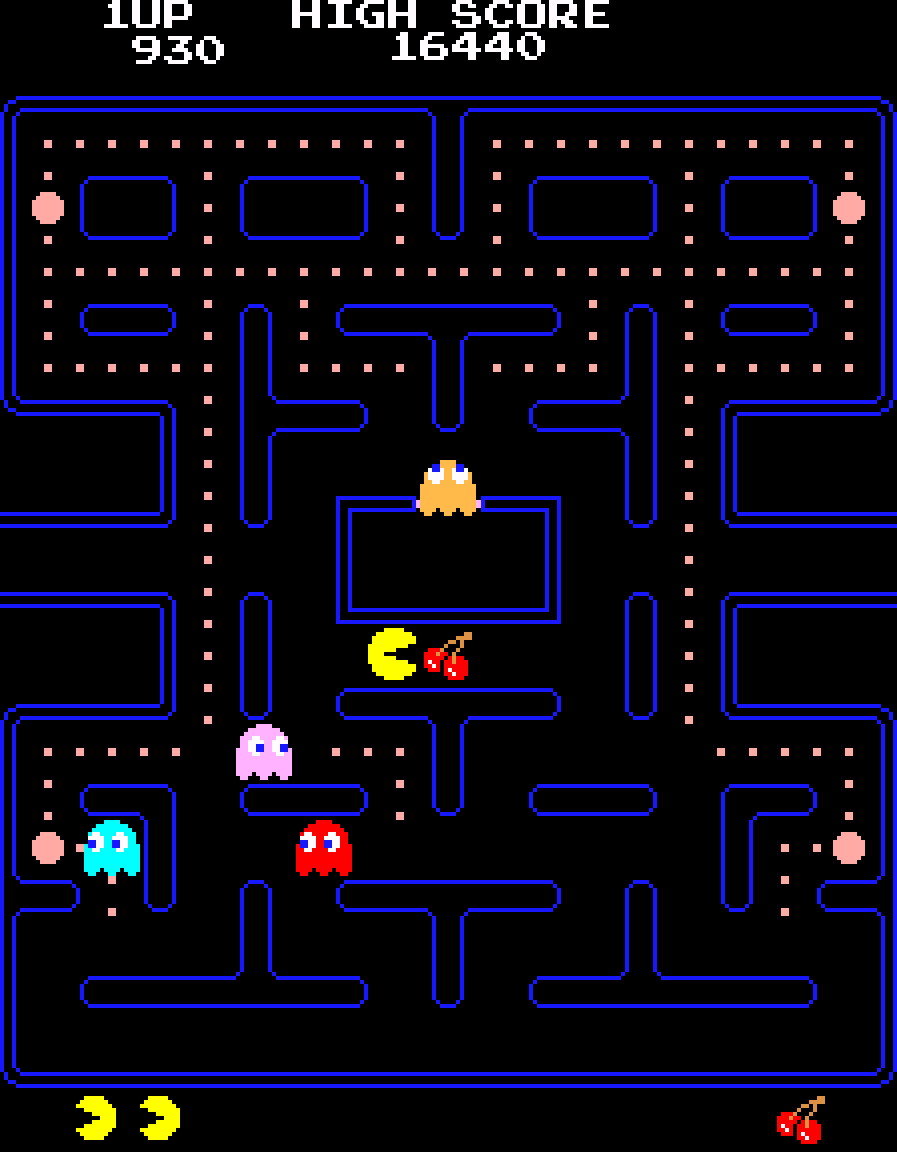
\includegraphics[scale=0.5]{../../pictures/pacman.jpg}
  \end{figure}

\end{column}
\begin{column}{0.5\textwidth}  %%<--- here

  \begin{figure}
  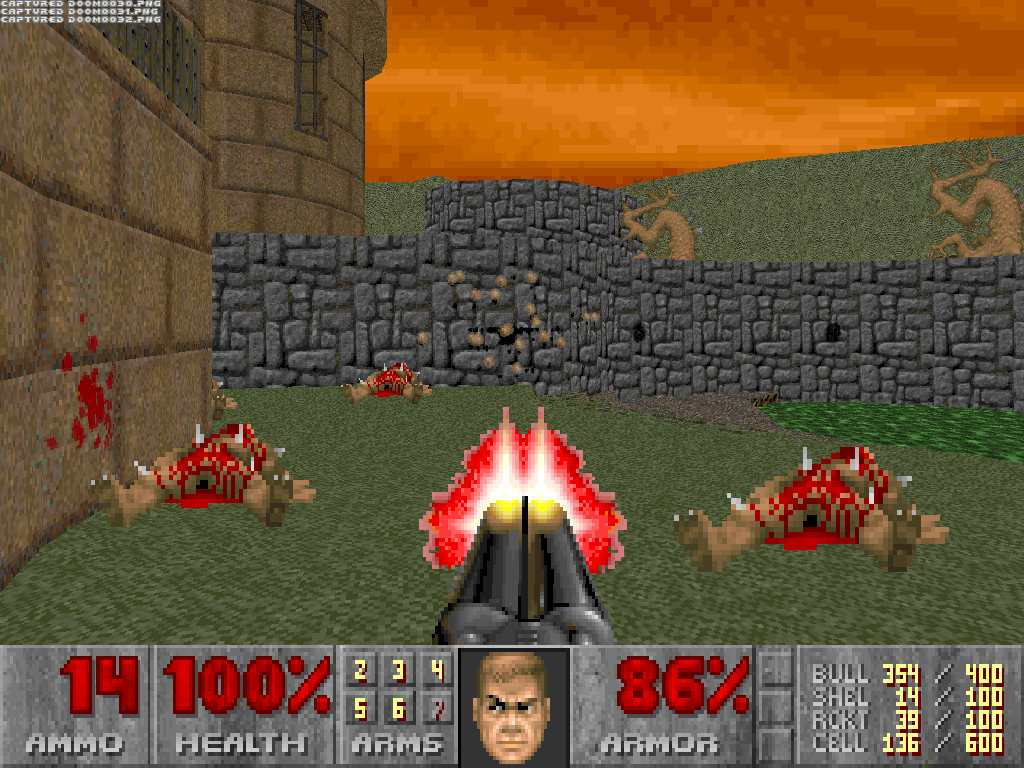
\includegraphics[scale=0.15]{../../pictures/doom.jpg}
  \end{figure}

\end{column}
\end{columns}

\vspace{-40pt}
\begin{figure}
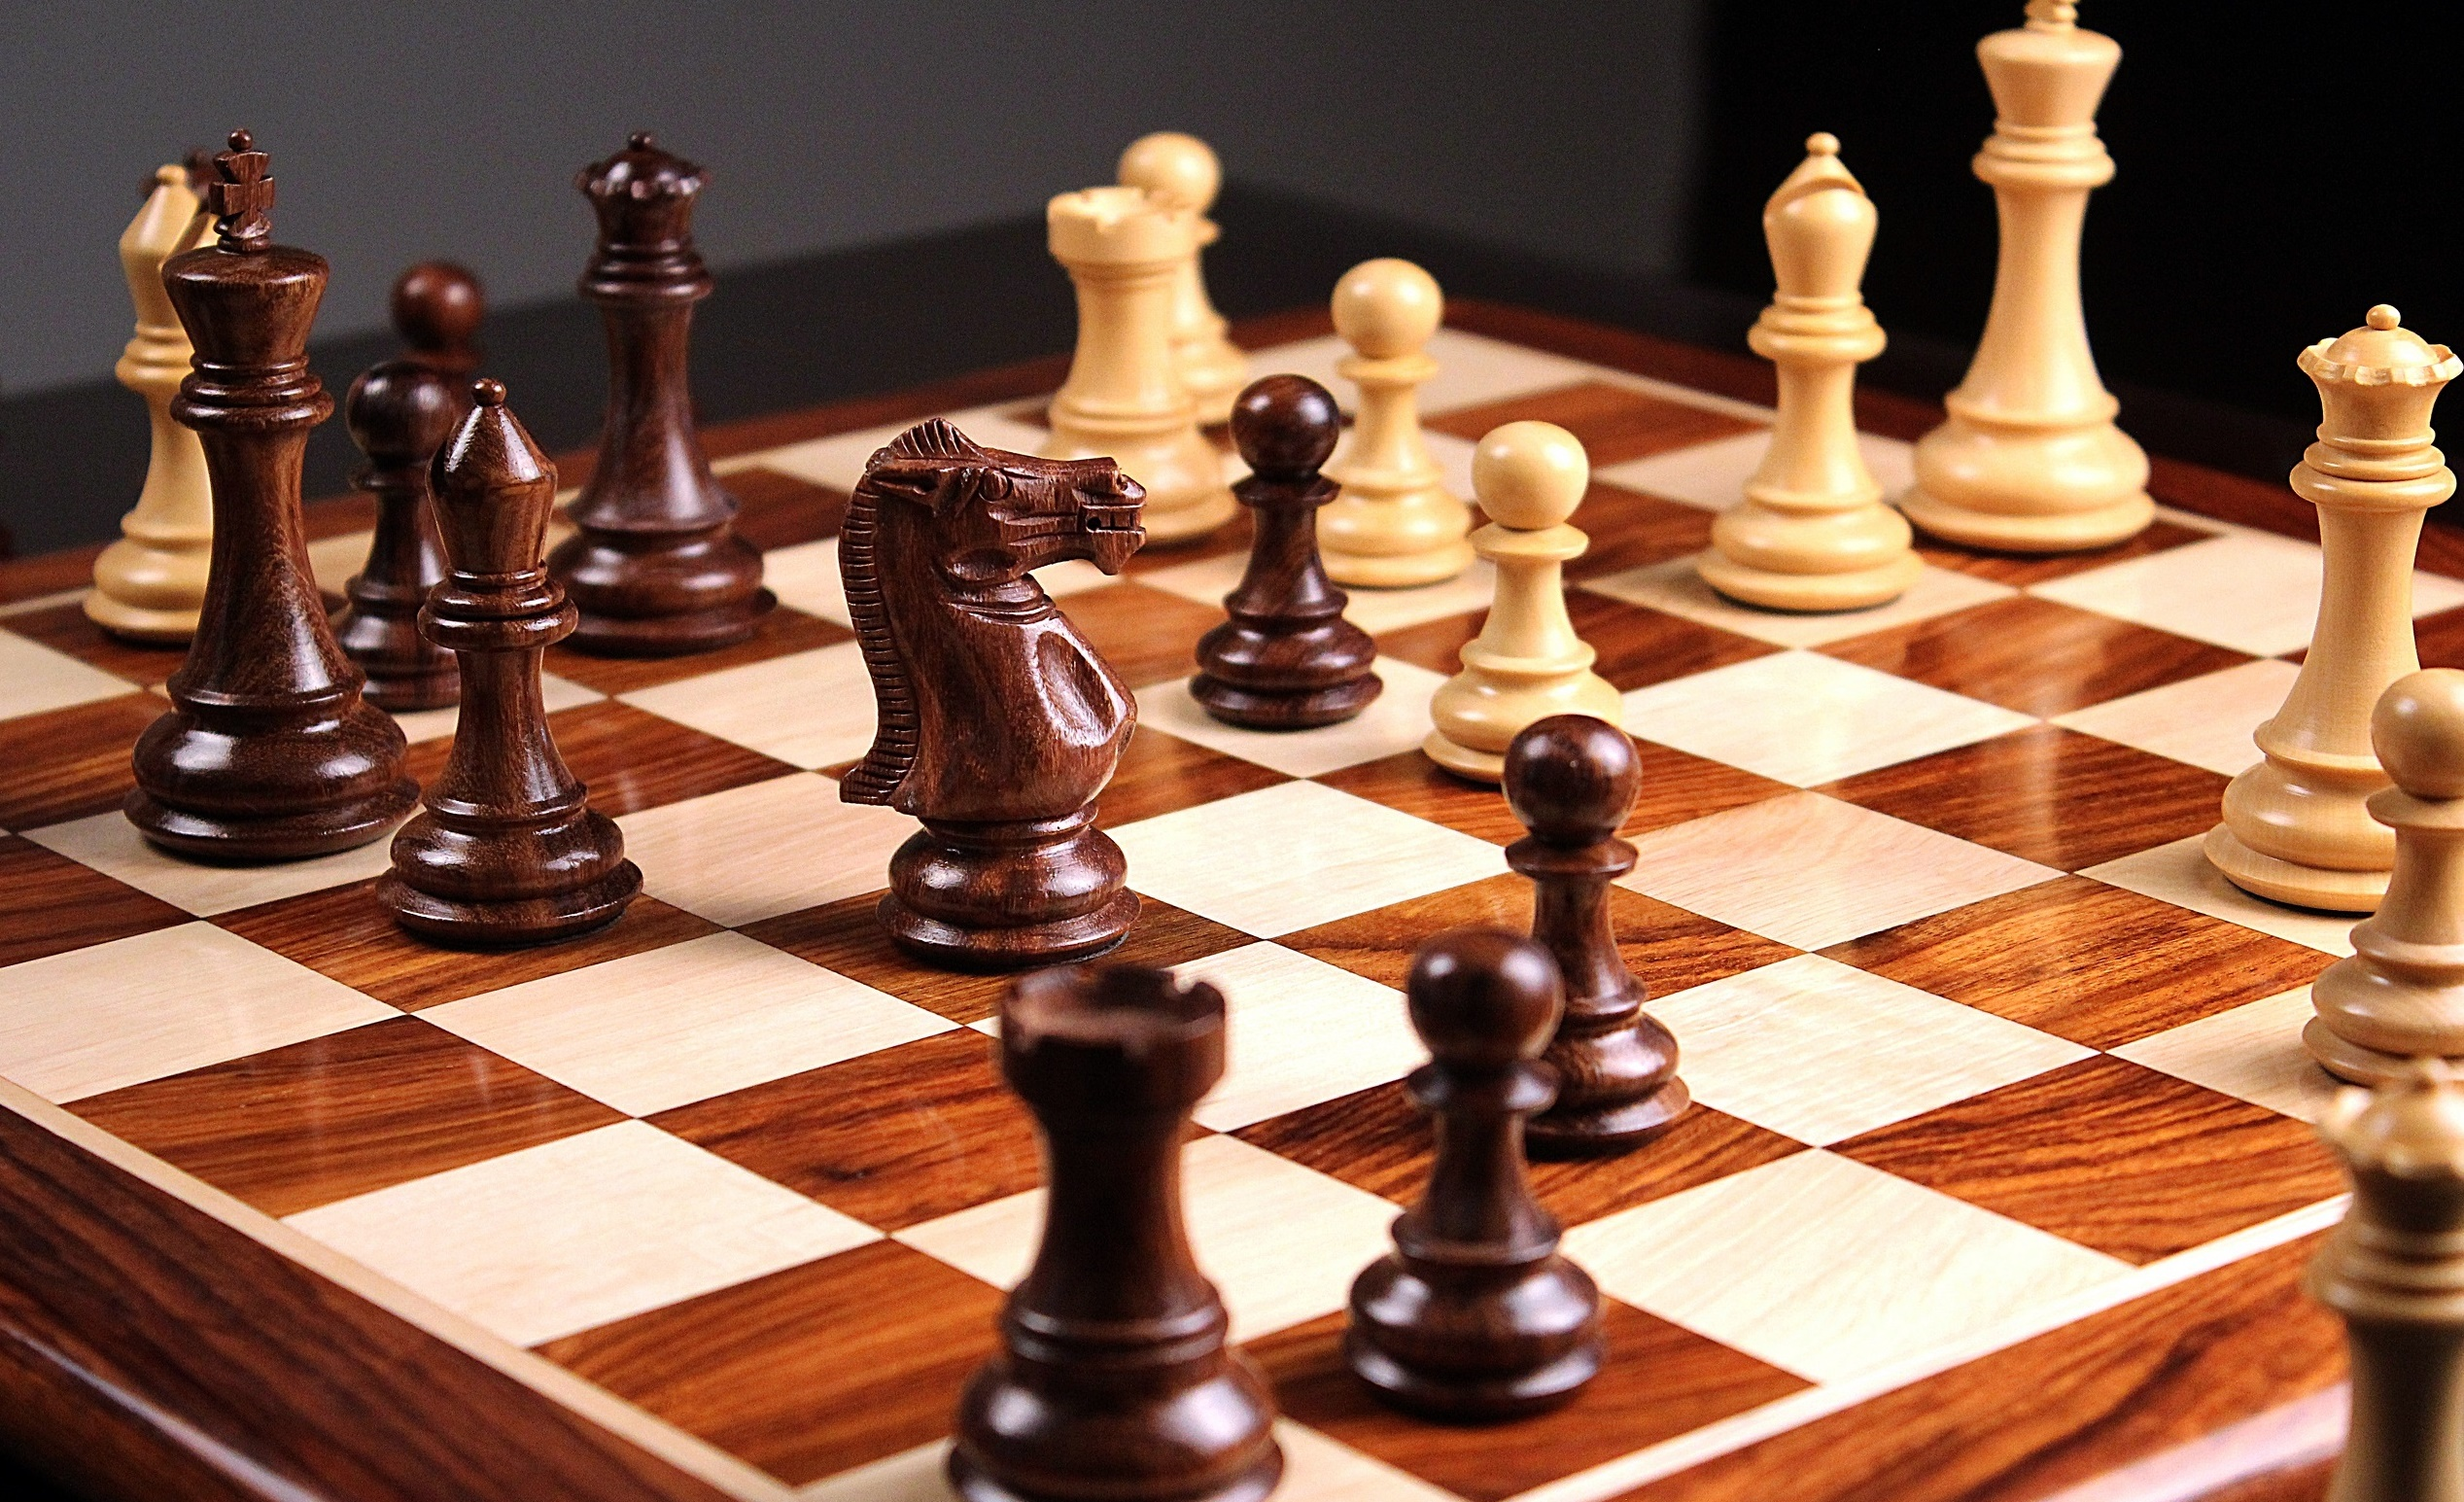
\includegraphics[scale=0.05]{../../pictures/chess.jpg}
\end{figure}

\end{frame}



\begin{frame}{\bf Reinforcement learning}

\begin{itemize}
  \item obtain {\bf state}
  \item choose {\bf action}
  \item {\bf execute} action
  \item obtain {\bf reward}
  \item learn from {\bf experiences}
\end{itemize}

  \begin{figure}
    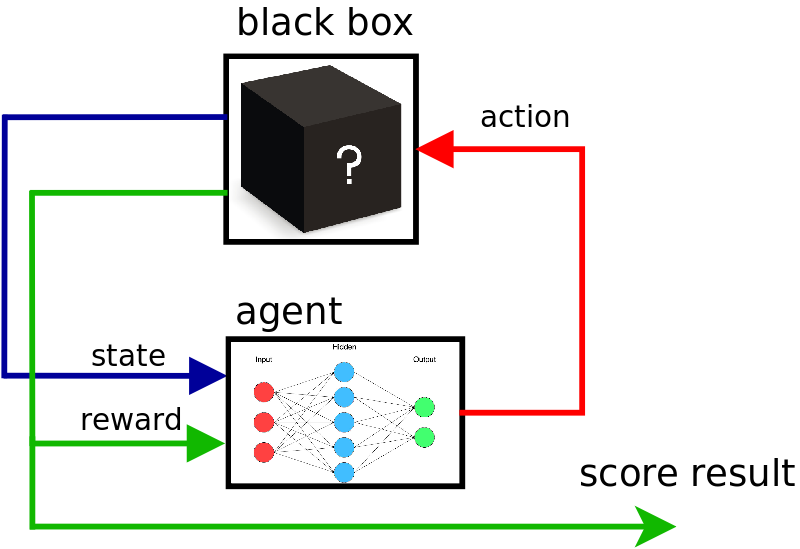
\includegraphics[scale=0.3]{../../diagrams/rl_mechanism.png}
  \end{figure}

\end{frame}

\begin{frame}{\bf Making decisions}

two possible strategies
\begin{itemize}
  \item strategy 1 : S0->S1, score = 1.0
  \item strategy 2 : S0->S2, score = 2.0
\end{itemize}

  \begin{figure}
    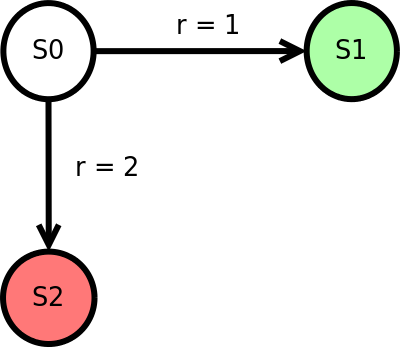
\includegraphics[scale=0.4]{../../diagrams/rl_trivial.png}
  \end{figure}

\end{frame}


\begin{frame}{\bf Making decisions}

two possible strategies, greedy = trap
\begin{itemize}
  \item strategy 1 : S0->S1, score = 1.0
  \item strategy 2 : S0->S2->S3, score = 2.0 + (-20.0) = -18
\end{itemize}

  \begin{figure}
    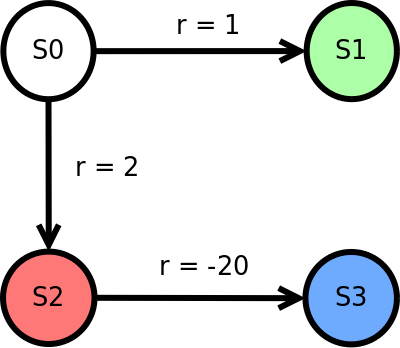
\includegraphics[scale=0.4]{../../diagrams/rl_trivial_trap.png}
  \end{figure}

\end{frame}



\begin{frame}{\bf Usefull links}

{\tiny
  \begin{thebibliography}{9}
    \bibitem {}ImageNet Classification with Deep Convolutional Neural Networks \url{https://papers.nips.cc/paper/4824-imagenet-classification-with-deep-convolutional-neural-networks.pdf}
    \bibitem {}Alex Krizhevsky web, \url{https://www.cs.toronto.edu/~kriz/}
    \bibitem {}Deep Belief Nets in C++ and CUDA C: Volume III \url{https://www.amazon.com/Deep-Belief-Nets-CUDA-Convolutional/dp/1530895189}
    \bibitem {}Deep Learning (Adaptive Computation and Machine Learning \url{https://www.amazon.com/Deep-Learning-Adaptive-Computation-Machine/dp/0262035618}
    \bibitem {}Densely Connected Convolutional Networks \url{https://arxiv.org/pdf/1608.06993.pdf}

    \bibitem {}MNIST dataset \url{http://yann.lecun.com/exdb/mnist/}
    \bibitem {}Digital signal processing for STM32 microcontrollers using CMSIS \url{https://www.st.com/resource/en/application_note/dm00273990.pdf}

    \bibitem {}CMSIS-NN: Efficient Neural Network Kernels for Arm Cortex-M CPUs \url{https://arxiv.org/pdf/1801.06601.pdf}

  \end{thebibliography}
}

\end{frame}


\begin{frame}{\bf Q\&A}

\begin{figure}
  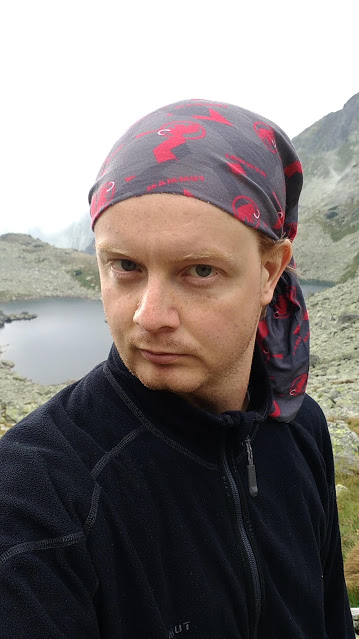
\includegraphics[scale=0.25]{../../pictures/me.jpg}
\end{figure}

\centering {
michal chovanec (michal.nand@gmail.com)
\url{www.youtube.com/channel/UCzVvP2ou8v3afNiVrPAHQGg}
}

\end{frame}


\end{document}




%% \bibitem {Deep Belief Nets in C++ and CUDA C: Volume III \url{https://www.amazon.com/Deep-Belief-Nets-CUDA-Convolutional/dp/1530895189}}
%% \bibitem {Deep Learning (Adaptive Computation and Machine Learning) \url{https://www.amazon.com/Deep-Learning-Adaptive-Computation-Machine/dp/0262035618}}
%% \bibitem {Densely Connected Convolutional Networks \url{https://arxiv.org/pdf/1608.06993.pdf}}
